\documentclass[9pt]{beamer}
\usepackage[utf8]{inputenc}
\usepackage{txfonts}
\usepackage[english]{babel}
\usepackage{xcolor}
\usepackage{iwona}
\usetheme{CambridgeUS}
\usecolortheme{beaver}

\setbeamertemplate{headline}{}
% \setbeamertemplate{frametitle}{\insertframetitle}
\setbeamertemplate{navigation symbols}{}

\setbeamertemplate{itemize item}{\scriptsize\raise1.25pt\hbox{\donotcoloroutermaths$\blacktriangleright$}}
\setbeamertemplate{itemize subitem}{\tiny\raise1.5pt\hbox{\donotcoloroutermaths$\blacktriangleright$}}
\setbeamertemplate{itemize subsubitem}{\tiny\raise1.5pt\hbox{\donotcoloroutermaths$\blacktriangleright$}}
\setbeamertemplate{enumerate item}{\insertenumlabel.}
\setbeamertemplate{enumerate subitem}{\insertenumlabel.\insertsubenumlabel}
\setbeamertemplate{enumerate subsubitem}{\insertenumlabel.\insertsubenumlabel.\insertsubsubenumlabel}
\setbeamertemplate{enumerate mini template}{\insertenumlabel}

% \setbeamertemplate{itemize items}[square]
% \setbeamertemplate{items}[square]


% \setbeamertemplate{footline}[page number]{}


\newcommand{\bluemph}[1]{\structure{\emph{#1}}}
\newcommand{\redemph}[1]{\alert{\emph{#1}}}
\newcommand{\bluebf}[1]{\structure{\textbf{#1}}}
\newcommand{\redbf}[1]{\alert{\textbf{#1}}}

\newcommand\denote[1]{\llbracket #1 \rrbracket}
\newcommand\fesi{Fe-Si}

%  Structure
\newenvironment{remark}{\footnotesize \begin{description}\item[\emph{Remark}:]}{\end{description}}

\title{Formal verification of hardware synthesis}%
\author[T. Braibant]{Thomas Braibant$^1$ \and Adam Chlipala$^2$}
\institute[Inria]{Inria$^1$ (Gallium) \qquad MIT CSAIL$^2$}
\date[04/2013]{Journées compilation}

\setbeamercovered{transparent}
\setbeamerfont{frametitle}{size={\normalsize}}

% \usepackage[T1]{fontenc}
\usepackage{amsmath}
\usepackage{amssymb}
\usepackage{amsthm}
\usepackage{mathpartir}

\usepackage{listings}
\usepackage{graphicx}
\definecolor{ltblue}{rgb}{0,0.4,0.4}
\definecolor{dkblue}{rgb}{0,0.1,0.6}
\definecolor{dkgreen}{rgb}{0,0.4,0}
\definecolor{dkviolet}{rgb}{0.3,0,0.5}
\definecolor{dkred}{rgb}{0.5,0,0}
\usepackage{lstcoq}
\usepackage{lstocaml}
\newenvironment{twolistings}%
{\noindent\begin{tabular*}{\linewidth}{@{}c@{\extracolsep{\fill}}c@{}}}%
{\end{tabular*}}

% \AtBeginSection[]
% {
%    \begin{frame}
%        \frametitle{Outline}
%        \tableofcontents[currentsection,currentsubsection]
%    \end{frame}
% }

\begin{document}
% \newcommand \blue[1]{{\color{red!80!black}{#1}}}
\newcommand \orange[1]{{\color{orange}{#1}}}
% \newcommand \red[1]{{\color{red}{#1}}}
% \newcommand \grey[1]{{\color{gray}{#1}}}
% \newcommand \green[1]{{\color{violet}{#1}}}
% \newcommand \white[1]{{\color{white}{#1}}}

\newcommand\parenthesis[1] {
  \begin{flushright}
    {\scriptsize \redemph{{{{ #1}}}}}
  \end{flushright}

}

\begin{frame}
  \center 
  \titlepage
\end{frame} 

%%%%%%%%%%%%%%%%%%%%%%%%%%%%%%%%%%%%%% 
\begin{frame}
  \frametitle{Context: formal verification of hardware}
  
  \begin{itemize}
  % \item  Formally verified everything:
  %   \begin{itemize}
  %   \item Compilers (CompCert [2006])
  %   \item Operating Systems (Gypsy [1989]; seL4 [2009])
  %   \item Static analysers
  %   \item \alert<2->{Hardware}
  %   \end{itemize}
    
  %   \pause
    
  \item Verifying hardware with theorem provers:
    \begin{itemize}
    \item many formalizations of hardware description languages (ACL2 , HOL, PVS)
      % ACL2 :DE2
      % Hol : Experience with embedding hardware description languages in HOL (1992)
      % PVS : Bluespec
    \item many models of hardware designs (ACL2, HOL, PVS, Coq) 
      \begin{itemize}
      \item[-] Floating-point operations verified at AMD using ACL2 
      \item[-] VAMP [2003]  (a pipelined micro-processor verified in PVS)
      \end{itemize}
    \item high-level formalization of the ARM architecture in HOL
    \item ...
    \end{itemize}

    \pause
    
    % This verification does not match what is really done
  \item Shift toward \alert{hardware synthesis}: 
    \begin{itemize}
    \item generates low-level code (RTL) from high-level HDLs
    \item argue (in)formally that this synthesis is correct
    \end{itemize}
    \parenthesis{Esterel, Lustre, System-C, Bluespec, \dots}
  \end{itemize}
\end{frame}

%%%%%%%%%%%%%%%%%%%%%%%%%%%%%%%%%%%%%% 
\begin{frame}
  \frametitle{This project}
  \begin{itemize}
  \item  Investigate verified hardware synthesis in Coq
    
    \begin{center}
      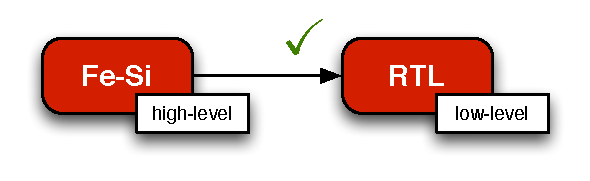
\includegraphics[height= 2cm ]{figs/compilation.pdf}
    \end{center}
    \pause
    
  \item Source language: \alert{\fesi{}} (Featherweight Synthesis)
    \begin{itemize}
    \item Stripped down and simplified version of \alert{Bluespec} 
    \item Semantics based on ``guarded atomic actions'' (with a flavour of transactional memory)
    \end{itemize}
    
    \pause
    
  \item Target language: RTL
    \begin{itemize}
    \item Combinational logic and next-state assignments for registers
    \item No currents, no delays, single-clock
    \end{itemize}
  \end{itemize}
\end{frame}

\begin{frame}[fragile]
  \frametitle{A certified compiler in a nutshell}
  \newcommand\behaviors[1]{{\mathcal B}\left(#1\right)}
  \begin{itemize}
  \item Define \alert{deep-embeddings}
    \begin{itemize}
    \item Define data-structures to represent programs (a prerequisite to write a compiler)
    \item Define what is a program's semantics 
    \end{itemize}
    
    \pause
    
  \item Implement the compiler

    \pause

  \item Pick a phrasing for semantic preservation:
    \begin{displaymath}
      \behaviors{P_1} \mathbin{\square} \behaviors{P_2} 
      \qquad  \begin{cases}
        \square \in \left\{\subseteq, \supseteq, \equiv \right\} \\
        \text{deterministic}~P_2 ? \\
        \text{safe}~P_1 ? \\
      \end{cases}
    \end{displaymath}

    \pause

  \item Prove semantic preservation for your compiler. 
    \pause \parenthesis{easier said than done}
  \end{itemize}  
\end{frame}

\begin{frame}[fragile]
  \frametitle{A problem with binders}
  
  \alert{Extra goals:}
  \begin{itemize}
  \item make it easy to write source programs inside Coq;
  \item make it relatively easy to reason about them. 
  \end{itemize}

  \alert{Problem: abstract syntax}
\begin{center}
\vspace{-1em}
  \begin{columns}
    \column{0.4\linewidth}
\begin{ocaml}
let x = foo in 
let y = f x in 
let z = g x y in 
z + x
\end{ocaml}
    \column{0.4\linewidth}
\begin{ocaml}
let foo in 
let f #1 in 
let g #2 #1 in 
#1 + #3
\end{ocaml}
\end{columns}
\end{center}

\pause 
\begin{itemize}
\item A complicated problem, many solutions, no clear winner;
\item Here, hijack Coq binders using Parametric Higher-Order
  Abstract Syntax (PHOAS)
\end{itemize}
\end{frame}

% \begin{frame}[fragile]
%   \frametitle{A PHOAS primer}
%   \framesubtitle{Face-off with Dependent de Bruijn indices}
%   \begin{columns}
%     \column{0.07 \linewidth}
%     \column{0.5 \linewidth}
% \newcommand\env{\Gamma}
% \begin{coq}
% Inductive var : list T -> T -> Type :=
% | 0 : forall $\env$ t , var (t::$\env$) t
% | S : forall $\env$ t u , var $\env$ u -> var (t::$\env$) u. 

% Inductive term : list T -> T -> Type :=
% | Var: forall $\env$ t, var $\env$ t -> term $\env$ t
% | Abs: forall $\env$ $\alpha$ $\beta$, term ($\alpha$:: $\env$) $\beta$ -> 
%            term $\env$ ($\alpha$ $\ulcorner \to \urcorner$ $\beta$)
% | App: ...  

% Example K := 
% $\quad$Abs (Abs (Var (S 0))).
% \end{coq}
%     \column{0.5 \linewidth}
% \only<2->{\phoasprimer}
%   \end{columns}
%   \begin{itemize}
%   \item<3> Two alternative  \alert{intrinsic approaches}
%     \begin{itemize}
%     \item strongly typed syntax
%     \item alternative to syntax + typing judgement
%     \end{itemize}
%   \end{itemize}
% \end{frame}

%%%%%%%%%%%%%%%%%%%%%%%%%%%%%%%%%%%%%% 

\begin{frame}
  \frametitle{Outline}       
  \tableofcontents  
\end{frame}

%%%%%%%%%%%%%%%%%%%%%%%%%%%%%%%%%%%%%% 

\section{A glimpse of the languages and the compiler}
\begin{frame}[fragile]
  \frametitle{\fesi{} abreviated}

  \fesi{} programs:
  \begin{itemize}
  \item update a set of \alert{memory elements} $\Phi$;
    \\
    \parenthesis{registers, register files, inputs, \dots}
  \item are based on \alert{guarded atomic actions} 
    \\
    \begin{center}
    \coqe{do n <- !x + 1; (y := 1; assert (n = 0)) orElse (y := 2)}      
    \end{center}
  \item are endowed with a (simple) \alert{synchronous semantics}
    \\
    \begin{center}
    \coqe{do n <- !x; x := n + 1; do m <- !x; assert (n = m)}
    \end{center}
  \end{itemize}
\end{frame}

\begin{frame}[fragile]
  \frametitle{\fesi{} in a nutshell}
  \begin{columns}
\column{0.05\linewidth}

\column{0.7 \linewidth}
\begin{coq}
Variable var: ty -> Type. 
Inductive expr: ty -> Type := ...

Inductive action: ty -> Type:=
| Return: forall t, expr t -> action t
| Bind: forall t u,  action  t -> (var t -> action u) -> action u
(** control-flow **)
| OrElse: forall t, action t -> action t -> action t
| Assert: expr B -> action unit    
(** memory operations on registers **)
| Read: forall t, (Reg t) $\in \Phi$ -> action t
| Writ: forall t, (Reg t) $\in \Phi$ -> expr t -> action unit
| ... 
\end{coq}
    \end{columns}
\begin{itemize}
\item Expressions are side-effects free. 
\item \vspace{-.5em}
  \begin{coq}
Definition Eval $\Phi$ t (a: forall V, action V t): $\denote\Phi$ -> option ($\denote{\tt t}$ * $\denote\Phi$).
\end{coq}
\end{itemize}

\end{frame}
%%%%%%%%%%%%%%%%%%%%%%%%%%%%%%%%%%%%%% 
\begin{frame}[fragile]
  \frametitle{RTL abreviated}
  
  An RTL circuit is abstracted as:
  \begin{itemize}
  \item a set of memory elements $\Phi$;
  \item a combinational next-state function.
  \end{itemize}
  
  \begin{center}
    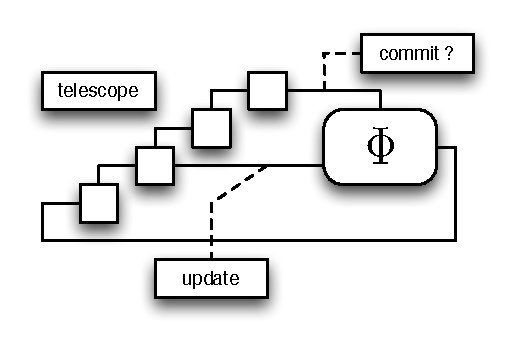
\includegraphics[width=5cm]{figs/rtl.pdf}  
  \end{center}

\end{frame}
%%%%%%%%%%%%%%%%%%%%%%%%%%%%%%%%%%%%%% 

% \defverbatim[colored]\firstpass{
% \begin{ocaml}
% x0 <-  ! r1;
% x1 <- x0 <> 0;
% x2 <-  !r2;
% x3 <- x0 - 1;
% x4 <- x2 + 1;
% x5 <-  !r2;
% x6 <- x6;
% begin 
%   if x1 then (r1 := x3; r2 := x4);
%   if  !x1 then (r1 := x6)
% end
% \end{ocaml}} 

% \defverbatim[colored]\secondpass{
% \begin{ocaml}
% x0   <-  ! r1;
% x1   <- x0 <> 0;
% x2   <-  ! r2;
% x3   <- x0 - 1;
% x4   <- x2 + 1;
% x5   <-  ! r2;
% x6   <- x5;
% x8   <- x1;
% x9   <- x1;
% x10 <- not x1;
% x11 <- x8 || x10;
% x12 <- x8 ?  x3 : x6;
% begin 
%   r1 := x12 when x11;
%   r2 := x4 when x9
% end
% \end{ocaml}} 

% \defverbatim[colored]\thirdpass{
% \begin{ocaml}
% x0   <- !r1 
% x1   <- 0;
% x2   <- x0 = x1;
% x3   <- not x2;
% x4   <- !r2;
% x5   <- 1;
% x6   <- x0 - x5;
% x7   <- x4 + x5;
% x8   <- !r2;
% x9   <- not x3;
% x10 <- x3 || x9
% x11 <-x3 ? x6 : x8
% begin
%   r1 := x11 when x10;
%   r2 := x8 when x3
% end
% \end{ocaml}}

% \defverbatim[colored]\finalpass{
% \begin{ocaml}
% x0   <- !r1 
% x1   <- 0;
% x2   <- x0 = x1;
% x3   <- not x2;
% x4   <- !r2;
% x5   <- 1;
% x6   <- x0 - x5;
% x7   <- x4 + x5;
% x8   <-x3 ? x6 : x4
% begin
%   r1 := x8 when true;
%   r2 := x4 when x3
% end
% \end{ocaml}}

% \begin{frame}[fragile]
%   \frametitle{Compiling \fesi{} to RTL}
  
% Running example:
% \begin{coq}
% do x <- ! r1;if (x <> 0) then {do y <- !r2; r1 := x - 1; r2 := y + 1} else { y <- !r2; r1 := y}
% \end{coq}
 
% \pause
% \begin{columns}
% \column{0.1 \textwidth}  
% \column{0.5 \textwidth}  
% \begin{enumerate}
% \item<+-> Pull out all bindings (that is, ANF)
% \item<+-> Push down the nested conditions
% \item<+-> Perform CSE (in 3-address code)
% \item<+-> WIP: Boolean simplification
% \end{enumerate}
% \column{0.5 \textwidth}  
% \only<2>{\firstpass}
% \only<3>{\secondpass}
% \only<4>{\thirdpass}
% \only<5>{\finalpass}
% \end{columns}
% \end{frame}

\begin{frame}
  \frametitle{A glimpse of the first-pass}
  
  \begin{itemize}
  \item Transform control-flow into data-flow.
  \end{itemize}

  \only<1>{
  \begin{center}
    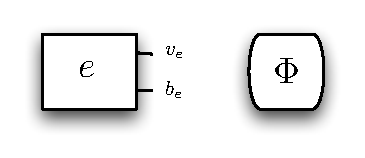
\includegraphics[width=5cm]{figs/compil-0.pdf}  
  \end{center}
}

\only<2-3>{
  \begin{itemize}
  \item Compiling \coqe{e orElse f}
  \end{itemize}
  \begin{center}
    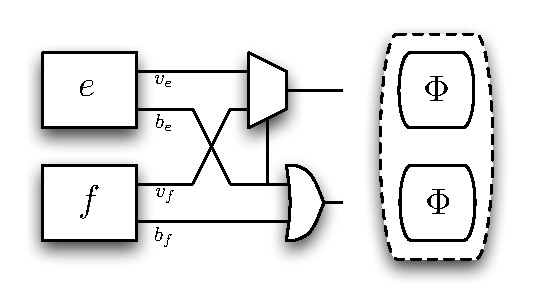
\includegraphics[width=7cm]{figs/compil-1.pdf}  
  \end{center}
}

\only<3>{
  \begin{itemize}
  \item  The $\Phi$ blocks are trees of effects on memory elements,
    that must be flattened.
  \end{itemize}
}
\end{frame}

\begin{frame}[fragile]
  \frametitle{Compiling \fesi{} to RTL}
  
  \begin{enumerate}
  \item Transform control-flow into data-flow programs (in A-normal form);
  \item Compute the update and commit values for each memory
    element;
  \item Perform syntactic common-sub-expression elimination;
  \item Perform Boolean expressions reduction using BDDs;
  \item Use an OCaml backend to generate Verilog code.
  \end{enumerate}

  \pause

  \begin{itemize}
  \item Steps [1-4] are proved correct in Coq.
    \parenthesis{Not a single lemma about substitutions!}
  \end{itemize}
\end{frame}

%%%%%%%%%%%%%%%%%%%%%%%%%%%%%%%%%%%%%% 
\section{Examples}

\begin{frame}
  \frametitle{Outline}       
  \tableofcontents [currentsection] 
\end{frame}

\begin{frame}
  \frametitle{Circuit generators}
  \begin{center}
    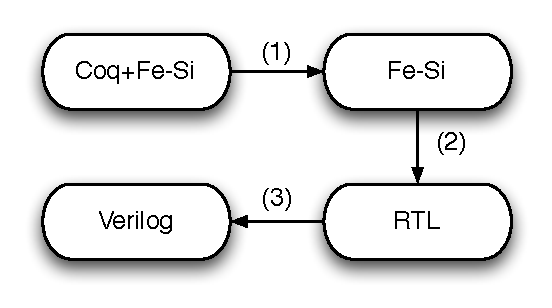
\includegraphics[width=5cm]{figs/examples.pdf}
  \end{center}
  \begin{enumerate}
  \item Coq's reduction (internal)
  \item Fe-Si to RTL (proved)
  \item RTL to Verilog (OCaml backend, trusted)
  \end{enumerate}
\end{frame}

\begin{frame}[fragile]
\frametitle{Recursive circuits: A von Neumann adder}
\begin{center}
  \only<1>{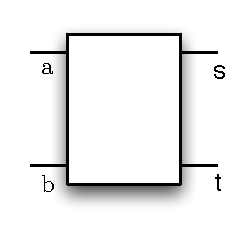
\includegraphics[height=3cm]{figs/adder-1.pdf}}
  \only<2>{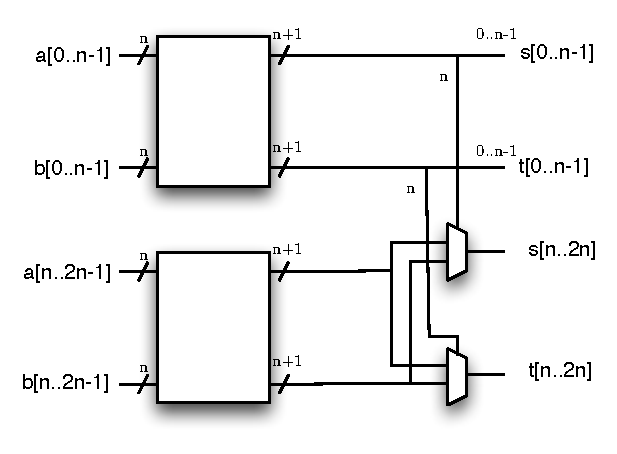
\includegraphics[height=6cm]{figs/adder-2.pdf}}
\end{center}
\begin{displaymath}
  s =  a + b \quad  t =  a + b + 1
\end{displaymath}
\end{frame}

\begin{frame}[fragile]
\frametitle{Recursive circuits: A von Neumann adder}
\framesubtitle{Meta-programming for free}
\begin{columns}
\column{0.1\linewidth}
\column{0.5\linewidth}
\begin{scoq}
Variable V : T -> Type. 

Fixpoint add $\Phi$ n (a : V (Tint [2^ n])) (b : V (Tint [2^ n])) := 
match n  with 
| 0 => ret ( (a = 1) || (b = 1) ;
                (a = 1) && (b = 1); a + b; a + b + 1)




$$
\end{scoq}
\column{0.5\linewidth}
\begin{scoq}
| S n => 
  do (aL,aH) <- (low a, high a);
  do (bL,bH) <- (low b, high b);
  do (pL, gL, sL, tL) <- add n aL bL; 
  do (pH, gH, sH, tH) <- add n aH bH; 
  do sH' <- (gL ? tH : sH);
  do tH' <- (pL ? tH : sH);
  do pH' <- (gH || (pH && gH));
  do gH' <- (gH || (pH && gL));
  ret (pH'; gH'; sL $\otimes$ sH' ; tL $\otimes$ tH' )
end.  
\end{scoq}
\end{columns}
\parenthesis{builds a 4-uple: carry-propagate, carry-generate, sum w/
  carry, sum w/o carry}
\pause
\begin{itemize}
\item Proof by induction on $n$
\end{itemize}
\end{frame}

\begin{frame}
  \frametitle{A bitonic sorter core}
  \begin{center}
    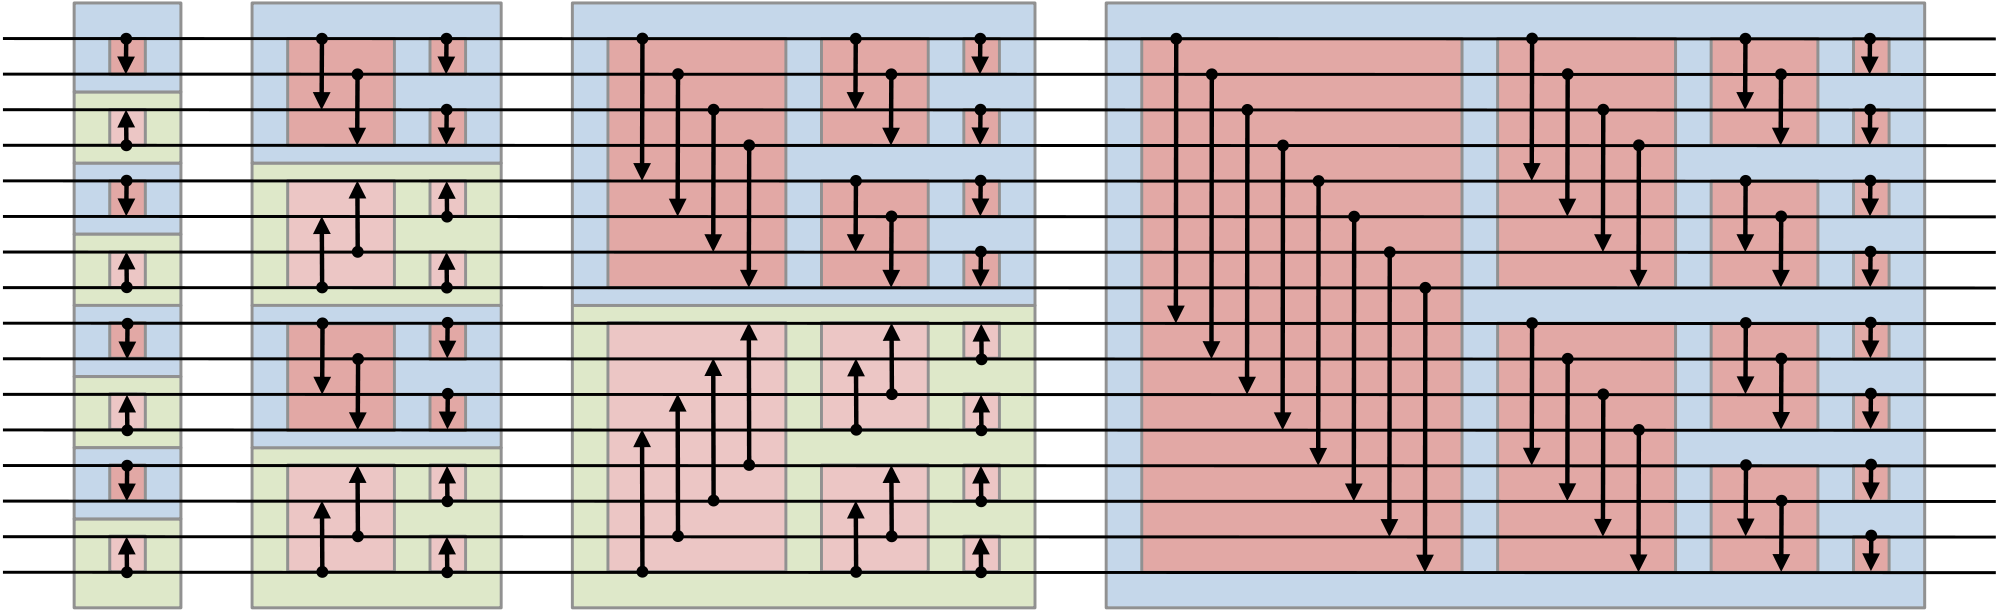
\includegraphics[width=\textwidth]{figs/bitonic1.png}
    \begin{itemize}
    \item Bitonic: $x_0 \le \dots \le x_k \ge \dots \ge x_{n-1}$ for
      some $k$, or a circular shift.
    \item Red: bitonic $\to$ $l_1$ bitonic, $l_2$ bitonic (and $l_1
      \le l_2$)
    \item Blue (resp. green): bitonic $\to$ sorted (resp. sorted in
      reverse order)
    \end{itemize}
  \end{center}
\end{frame}

\begin{frame}[fragile]
  \frametitle{A bitonic sorter code}
\newcommand\rebind{\leftsquigarrow}
  \begin{columns}
\column{0.5\linewidth}
  \begin{coq}
Fixpoint merge {n}: T n -> C n := 
match n with 
| 0 => fun t => ret (leaf t)
| S k => fun t => 
  do a,b  $\rebind$  min_max_swap (left t) (right t);
  do a <- merge a;
  do b <- merge b;
  ret (mk_N  a b)
end.
$ $\end{coq}
\column{0.5\linewidth}
\begin{coq}
Fixpoint sort {n} : T n -> C n :=
match n with 
| 0 => fun t => ret (leaf t)
| S n => fun t => 
  do l <- sort (left t); 
  do r $\rebind$ sort (right t);
  do r <- reverse r;                 
  do x $\rebind$ ret (mk_N l r);
  merge x
end\end{coq}
  \end{columns}
  \begin{itemize}
  \item \coqe{merge} builds the blue/green boxes
  \item \coqe{min_max_swap} builds the red boxes
  \end{itemize}

\pause
\begin{theorem}
Let $I$ be a sequence of length $2^n$ of integers of size $m$. The
circuit always produces an output sequence that is a sorted permutation of $I$.
\end{theorem}
\end{frame}


\begin{frame}
  \frametitle{A (family) of stack machines}
\begin{small}
  \begin{columns}
\column{0.2\linewidth}
    \begin{tabular}{rcll}
i & ::=   & \texttt{const $n$                     }\\
  & $|$   & \texttt{var   $x$                              }\\
  & $|$   & \texttt{setvar  $x$                            }\\
  & $|$   & \texttt{add                                        }\\
  & $|$   & \texttt{sub                                        }\\
  & $|$   & \texttt{bfwd $\delta$             }\\
  & $|$   & \texttt{bbwd $\delta$              }\\
  & $|$   & \texttt{bcond $c$ $\delta$ }\\
 \\
  & $|$   & \texttt{halt                                       }\\
\end{tabular}

\column{0.7\linewidth}
\begin{tabular}{ll}
$\vdash pc,\sigma,s \to pc+1, n :: \sigma,s$& \\
$\vdash pc,\sigma,s \to pc+1, s(x) :: \sigma,s$ & \\
$\vdash pc,v::\sigma,s \to pc+1, \sigma,s[x \leftarrow v]$ & \\
$\vdash pc,n_2::n_1::\sigma,s \to pc+1, (n_1+n_2)::\sigma,s$&\\
$\vdash pc,n_2::n_1::\sigma,s \to pc+1, (n_1-n_2)::\sigma,s$&\\
$\vdash pc,\sigma,s \to pc+1+\delta, \sigma,s$ &  \\
$\vdash pc,\sigma,s \to pc+1-\delta, \sigma,s$ & \\
$\vdash pc,n_2::n_1::\sigma,s \to pc+1+\delta, \sigma,s$ & \text{if $c~n_1~n_2$} \\
$\vdash pc,n_2::n_1::\sigma,s \to pc+1, \sigma,s$ & \text{if  $\neg (c~n_1~n_2)$} \\
\texttt{no reduction}
\end{tabular}
\end{columns}
\end{small}

\begin{itemize}
\item Implementation parameterized by the size of the values, the size of the
  stack, \dots
\end{itemize}
\end{frame}

\begin{frame}[fragile]
  \frametitle{Stack machine excerpt}
  \begin{columns}
\column{0.4\linewidth}
\begin{coq}
Definition pop :=
do sp <- ! SP;       
do v <- read STACK [: sp - 1];
do _ <- SP ::= sp - 1;
ret v.    
\end{coq}
\column{0.4\linewidth}
\begin{coq}
Definition Isetvar pc x := 
do v <- pop; 
do _ <- write REGS [: x <- v];
PC ::= pc + 1.
$ $
\end{coq}
  \end{columns}
  \begin{displaymath}
\vdash pc,v::\sigma,s \to pc+1, \sigma,s[x \leftarrow v]
  \end{displaymath}
  \begin{itemize}
  \item Combine these pieces of code using a \coqe{case} construct
  \item Prove the Fe-Si implementation correct w.r.t. the previous semantics
  \end{itemize}
\end{frame}
%%%%%%%%%%%%%%%%%%%%%%%%%%%%%%%%%%%%%% 
\begin{frame}[fragile]
  \frametitle{Meta-programming at work}

  \begin{itemize}
  \item Recursive circuits. 
  \item \alert{Combinators and schedulers} of atomic actions.
  \item In these cases, using Coq as a meta-language makes it possible
    to prove things. 
  \end{itemize}
\end{frame}
%%%%%%%%%%%%%%%%%%%%%%%%%%%%%%%%%%%%%% 


\section{Conclusion}
% Rant about Coq
\begin{frame}
  \frametitle{Outline}       
  \tableofcontents [currentsection] 
\end{frame}

\begin{frame}[fragile]
  \frametitle{Some remarks}
  \begin{itemize}

  \item Stepping back
    \begin{itemize}
    \item Bluespec started as an HDL deeply embedded in Haskell
    \item Lava [1998] is another HDL deeply embedded in Haskell
    \item \fesi{} is ``just'' another HDL,  deeply embedded in \alert{Coq}
      \pause
      \begin{itemize}
      \item semantics (i.e., interpreter), compiler and programs are \alert{integrated seamlessly}
      \item dependent types capture some interesting properties in
        hardware
      \item use of extraction to dump compiled programs
      \end{itemize}
    \end{itemize}

    \pause
    
  \item Future work
    \begin{itemize}
    \item Improve on the language (FIFOs, references).
    \item Make the compiler more realistic (automatic scheduling of
      atomic actions).
    \item Embed a DSL for floating-point cores? 
    \end{itemize}
    
    \pause

  \item Take-away message
    \begin{itemize}
    \item Coq can be used as an embedding language for DSLs!
    \end{itemize}
    
  \end{itemize}
\end{frame}

\begin{frame}
  \frametitle{Thank you for your attention}
  
  \begin{center}
    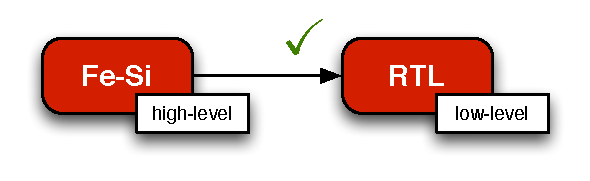
\includegraphics[height= 2cm ]{figs/compilation.pdf}

    \vspace{1cm}

    If you have any questions ... \\
  \end{center}
  
\end{frame}
\end{document}


\defverbatim[colored]\phoasprimer{
}
\begin{frame}[fragile]
  \frametitle{A PHOAS primer}
  \begin{itemize}
  \item Use Coq bindings to represent the bindings of the object language.
    \newcommand\arrow{\ulcorner \to \urcorner}
\begin{coq}
Section t. 
  Variable var: T -> Type.
  
  Inductive term : T -> Type :=
  | Var: forall t, var t -> term t
  | Abs: forall $\alpha$ $\beta$, (var $\alpha$ -> term $\beta$) -> term ($\alpha$ $\arrow$ $\beta$)
  | App: ...
End t. 

Definition Term := forall (var: T -> Type), term var. 

Example K $\alpha$ $\beta$ : Term ($\alpha~\arrow{}~\beta{}~\arrow{}~\alpha$):= fun V =>
$\quad$Abs (fun x => Abs (fun y => Var x)).
\end{coq}

\pause

\item An \alert{intrinsic approach} (strongly typed syntax vs. syntax + typing judgement)
\end{itemize}
\end{frame}
